
\section{Implementation}


\subsection{Operation}
Text editing can be realized with only two operations. 
 - Insert
 - Delete
 - Split

All operations have some equivalent properties. They must provide a function called \texttt{inverse()} that returns the inverse operation, a . 

They are represented by the Operation Interface.
 
\subsubsection{Operation Hierarchy}
\begin{figure}[H]
\centering
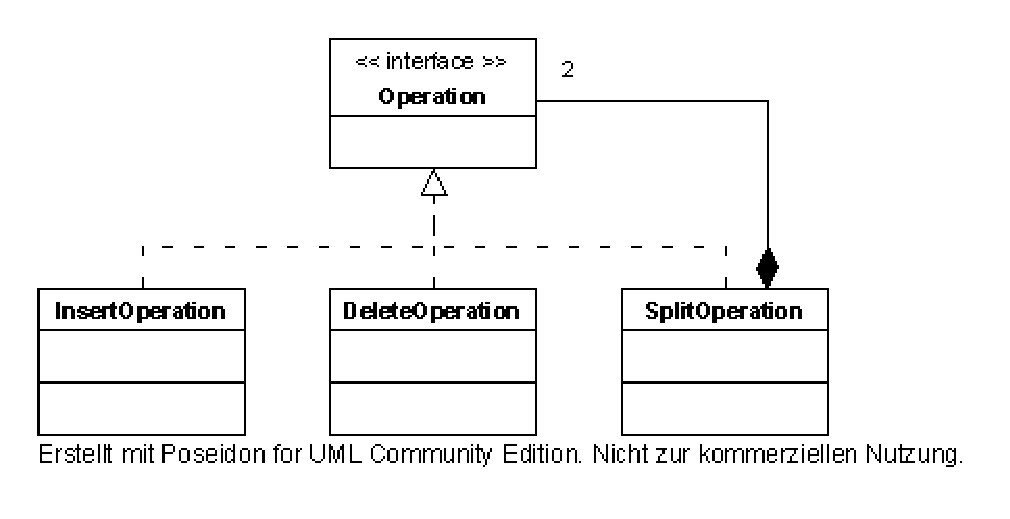
\includegraphics[height=4cm,width=8cm]{../../images/algo-impl/operation.eps}
\caption{Operation Hierarchy}
\end{figure}

\subsubsection{InsertOperation}


\subsubsection{DeleteOperation}
\subsubsection{SplitOperation}
\label{Split_Operation}
  - no operation
  - wrapper to handle special cases -> \ref{Delete_Insert}


\subsection{Request}

\newpage
\subsection{GOTO Transformation Functions}

\subsubsection{Overview}
The GOTO (generic operation transformation optimized) transformation functions are designed to work with strings. The advantage is that less transformations are needed when a string has been inserted into a text. To understand the exigence of transformation functions see \emph{Evaluation Algorithms}.

The inclusion transformation functions are used to check the influence of a given operation B to another operation A. If so, the operation A will be transformed into operation A'. To transform an operation means to adapt position and text of the operation. In the majority of cases this is a very simple process. But sometimes it is necessary to extract a text fragment or to split up an operation in two parts. For more details about splitting operations into two parts see \ref{Split_Operation}.

All possible transformations \emph{cases} with two insert/delete operations are represented by figure \ref{Transformation Overview} and explained in the following sections:
%\begin{figure}[H]
%\centering
%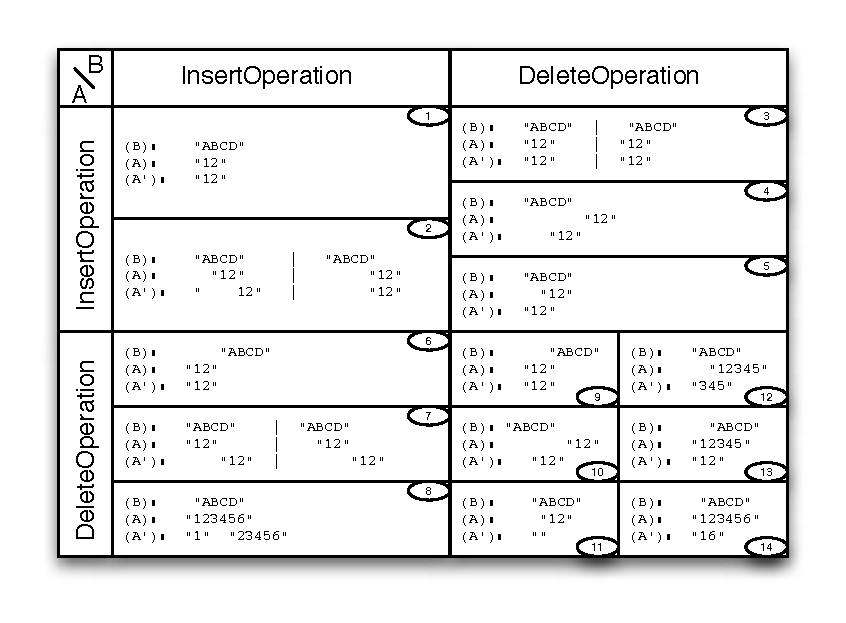
\includegraphics[height=12cm,width=16cm]{../../images/algo-impl/transform_overview.eps}
%\caption{Transformation Overview}
%\label{Transformation Overview}
%\end{figure}

\subsubsection{Insert/Insert}
\begin{itemize}
\item \textbf{Case 1:}
Operation A starts before operation B. Nothing has to be transformed.
\item \textbf{Case 2:}
Operation A starts in or behind operation B. Index of operation A' must be increased by the length of the text of operation B.
\item \textbf{Special case:}
It can occur that two insert operations (for example \texttt{Ins(1,'a')} and \texttt{Ins(1,'b')}) have the same position. How should the correct transformation looks like (has the insertion of 'a' to be before or after 'b')? This is an undecidable problem. Therefore some extra rules must be defined. The first approach to solve this problem is by prefering the operation with the lower ascii value. With this method the final text would be \texttt{ab}. The following figure demonstrates that this solution can violate the user intention:
\begin{figure}[H]
\centering
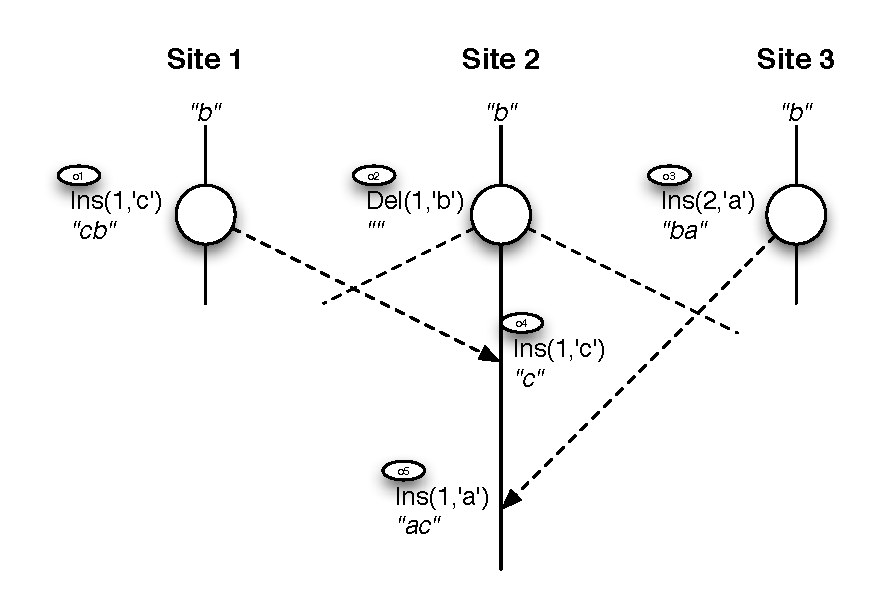
\includegraphics[height=5cm,width=8cm]{../../images/algo-impl/transform_ins_ins_char.eps}
\caption{Insert based on character ord}
\label{Insert based on character ord}
\end{figure}
DESCRIPTION

The second approach is working with some exrta informations. If an operation has been generated the original position is saved too. Adapted to the scenario in figure \ref{Insert based on character ord} the insert operation of site 1 would looks like \texttt{Ins(1,'a',1)}. Similar to the insert operation of site 1 the insert operation of site 3 would looks like \texttt{Ins(2,'b',2)}. The added third parameter representing the original position. After an insert operation has been generated the position and the original position have the same value. The differece of the two positions is shown after a transfomation. Unlike the position (first parameter) the original position will never be transformed/changed and remains with the original value.
Now site 1 sends the request \texttt{Ins(1,'c',1)} to site 2. After site 2 received the request, site 3 sends the request \texttt{Ins(2,'a',2)} to site 2. On site 2 this request will be first transformed with \texttt{Del(1,'b')} into \texttt{Ins(1,'a',2)}. This is necessary because while site 3 was generating the request, site 2 deleted the character \texttt{b}. After this transformation the new request have to be transformed with the request from site 1. This transformation would looks like: \texttt{transform( Ins(1,'a','2'), Ins(1,'c',1))}. This means that the effect from the operation \texttt{Ins(1,'c',1)}) will be included into operation \texttt{Ins(1,'a',2)}. The problem to solve now is the same as before, but with the extra information its not longer infeasible. After detecting that the two operations have the same position the transformation function compares the original positions. With this solution the \texttt{c} will be inserted before the \texttt{a} and the user intention is preserved.


  - origin
    - problem
\begin{figure}[H]
\centering
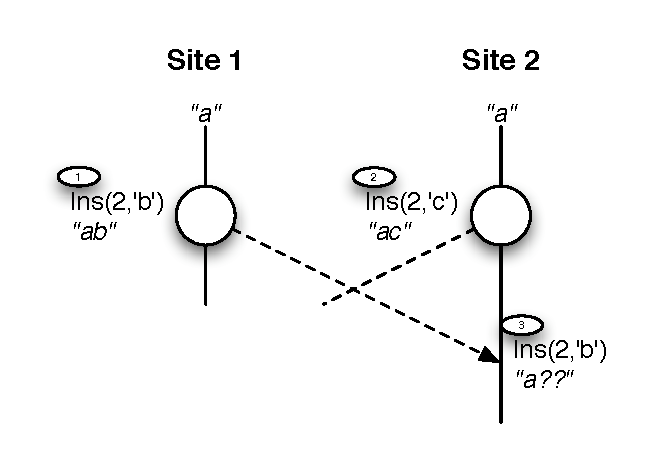
\includegraphics[height=3.5cm,width=5cm]{../../images/algo-impl/transform_ins_ins_origpos.eps}
\caption{Insert based on original positions}
\label{Insert based on original positions}
\end{figure}
  - isTransformOpPrivileged
\end{itemize}

\subsubsection{Insert/Delete}
\begin{itemize}
\item \textbf{Case 3:}
Operation A starts before or at the same position as operation B. Nothing has to be transformed.
\item \textbf{Case 4:}
Operation A starts after operation B. Index of operation A' must be reduced by the length of the text of operation B.
\item \textbf{Case 5:}
Operation A starts in operation B. Index of A' must be the index of operation B.
\end{itemize}

\subsubsection{Delete/Insert}
\begin{itemize}
\item \textbf{Case 6:}
Operation A is completly before operation B. Nothing has to be transformed.
\item \textbf{Case 7:}
Operation A starts before or at the same position as operation B. Index of operation A' must be increased by the length of the text of operation B.
\item \textbf{Case 8:}
Operation B is in the range of operation A. Operation A' must be splitted into two delete operations. For more details about this process see \cite{Split_Operation}.
\end{itemize}

\subsubsection{Delete/Delete}
\begin{itemize}
\item \textbf{Case 9:}
Operation A is completly before operation B. Nothing has to be transformed.
\item \textbf{Case 10:}
Operation A starts at the end or after operation B. Index of operation A' must be reduced by the length of the text of operation B.
\item \textbf{Case 11:}
Operation A and operation B are overlapping. Operation B starts before or at the same position as operation A and ends after or at the same position as operation A. Content of operation A has been allready deleted by operation B. Nothing has to be deleted by operation A. A' is called a noop (no-operation).
\item \textbf{Case 12:}
Operation A and operation B are overlapping. Operation B starts before or at the same position as operation A and ends before operation A. The overlapping part of the two operations has been deleted by operation B. Operation A' has to delete only the remaining text (text after the overlapping text of the two operations).
\item \textbf{Case 13:}
Operation A and operation B are overlapping. Operation B starts after operation A and ends after or at the same position as operation A. The overlapping part of the two operations has been deleted by operation B. Operation A' has to delete the remaining text (text before the overlapping text of the two operations).
\item \textbf{Case 14:}
Operation A and operation B are overlapping. Operation B is fully in operation A. The overlapping part of the two operations has been deleted by operation B. Operation A' has to delete the remaining text (text before and after the overlapping text of the two operations).
\end{itemize}



\subsection{Client}


\subsection{Server}


\subsection{Undo/Redo}


\subsection{Tests}

